%!TEX root = ../report.tex

\begin{document}
    \chapter{Methodology}

    \section{Pipeline Workflow: 3D Lane Detection }
        
        \subsection{3D Lane Geometry}
        In this section we will introduce the geometric representation of lanes in 3D space, image plane and birds eye view via the means of the transformation from one space to another. 
        
         \begin{figure}[h]
    \centering
    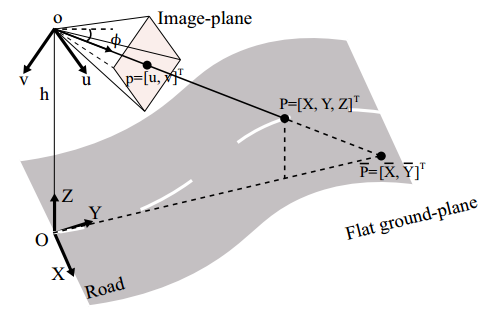
\includegraphics[width=9cm, height=5cm]{images/3d_lane_geometry.png}
    \caption{Geometric representation of lane point in 3D world space, image plane and virtual top view \cite{DBLP:journals/corr/abs-2112-15351}}
    \end{figure}
    
    In the above figure the point $\textbf{P} =[X, Y, Z]^{T}$ is in 3D space and when it is projected onto the image plane it is defined by $\textbf{p} = [u, v]^{T}$. Birds eye view can be seen as the projection of point $\textbf{P}$ from 3D space to flat ground plane, where $Z=0$. $\textbf{O}$ is the origin of the 3D space which is obtained by projecting the origin of camera center $\textbf{o}$ on to the flat ground plane with $Z = 0$. The focal length and other intrinsic parameters of the camera is fixed, where as the orientation of the camera in terms of camera height \textbf{h}  and camera pitch \textbf{$\phi$} is fixed or sometimes it is predicted from the network. 
    
    Using geometric transformation and homography as discussed above we can project points in 3D space to virtual flat ground plane. As per the figure 4.1 we can say that the point \textbf{P} it projection on image plane and flat ground plane, all lies on the same ray and this co-linear relationship will hold even if when there are downhill scenarios where $Z<0$.  
    
    
    
        
        \subsection{Architecture: 1}
        
        \subsection{Architecture: 2}
        \subsubsection{Stage 1: Image Segmentation}
        \subsubsection{Stage 2: Semi-Local 3D Lane Detection}
    
    \subsection{Loss Functions}
        (Write in general mentioning the sections which loss functions is used for what)
        
    \subsection{Experimental setup}
        \subsubsection{Datasets Used}
        \subsubsection{Evaluation Metrics}
        \subsubsection{Implementation Details}
    
    \section{Pipeline Workflow: 3D Lane AuxNet}
        \subsection{Architecture}
        \subsection{Dataset Used}
        \subsection{Evaluation Metrics}
        \subsection{Implementation Details}
        
\end{document}
